% Byte range diagram: multi-signature nesting (Chapter 13)
\documentclass[border=10pt]{standalone}
\usepackage{tikz}
\usetikzlibrary{positioning, decorations.pathreplacing, calc}
\usepackage{fontspec}
\setmainfont{Noto Serif}
\setsansfont{Noto Sans}
\setmonofont{DejaVu Sans Mono}[Scale=0.85]
\usepackage{xcolor}
\definecolor{sig1}{HTML}{bbdefb}
\definecolor{sig2}{HTML}{c8e6c9}
\definecolor{sig3}{HTML}{fff9c4}
\definecolor{gap}{HTML}{ffcdd2}
\definecolor{accent}{HTML}{0f3460}

\begin{document}
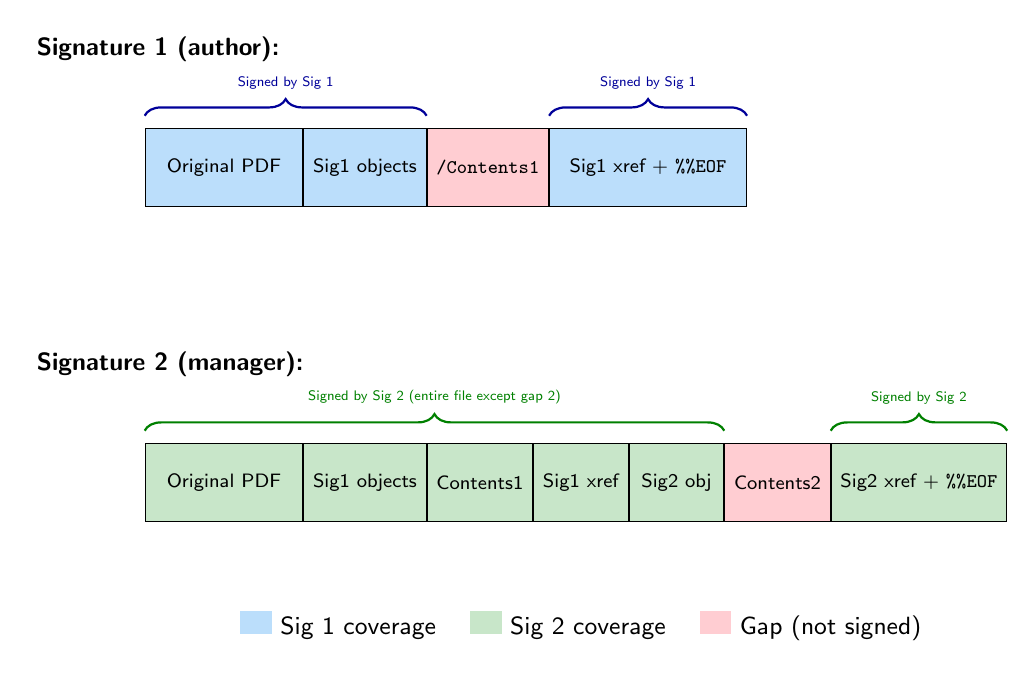
\begin{tikzpicture}[
    block/.style={draw, minimum height=1cm, text centered, font=\sffamily\scriptsize},
    brace/.style={decorate, decoration={brace, amplitude=6pt, mirror}},
    braceup/.style={decorate, decoration={brace, amplitude=6pt}},
]

% ── Signature 1 ──
\node[font=\sffamily\bfseries\small, anchor=west] at (0, 1.5) {Signature 1 (author):};

\node[block, fill=sig1, minimum width=2cm] (s1a) at (2.5, 0) {Original PDF};
\node[block, fill=sig1, minimum width=1.5cm, right=0pt of s1a] (s1b) {Sig1 objects};
\node[block, fill=gap, minimum width=1.5cm, right=0pt of s1b] (s1c) {\texttt{/Contents1}};
\node[block, fill=sig1, minimum width=2.5cm, right=0pt of s1c] (s1d) {Sig1 xref + \texttt{\%\%EOF}};

\draw[braceup, thick, blue!60!black] ($(s1a.north west) + (0,0.15)$) -- node[above=6pt, font=\sffamily\tiny, text=blue!60!black] {Signed by Sig 1} ($(s1b.north east) + (0,0.15)$);
\draw[braceup, thick, blue!60!black] ($(s1d.north west) + (0,0.15)$) -- node[above=6pt, font=\sffamily\tiny, text=blue!60!black] {Signed by Sig 1} ($(s1d.north east) + (0,0.15)$);

% ── Signature 2 ──
\node[font=\sffamily\bfseries\small, anchor=west] at (0, -2.5) {Signature 2 (manager):};

\node[block, fill=sig2, minimum width=2cm] (s2a) at (2.5, -4) {Original PDF};
\node[block, fill=sig2, minimum width=1.5cm, right=0pt of s2a] (s2b) {Sig1 objects};
\node[block, fill=sig2, minimum width=1.2cm, right=0pt of s2b] (s2c) {\scriptsize Contents1};
\node[block, fill=sig2, minimum width=1.2cm, right=0pt of s2c] (s2d) {Sig1 xref};
\node[block, fill=sig2, minimum width=1.2cm, right=0pt of s2d] (s2e) {Sig2 obj};
\node[block, fill=gap, minimum width=1.2cm, right=0pt of s2e] (s2f) {\scriptsize Contents2};
\node[block, fill=sig2, minimum width=1.8cm, right=0pt of s2f] (s2g) {Sig2 xref + \texttt{\%\%EOF}};

\draw[braceup, thick, green!50!black] ($(s2a.north west) + (0,0.15)$) -- node[above=6pt, font=\sffamily\tiny, text=green!50!black] {Signed by Sig 2 (entire file except gap 2)} ($(s2e.north east) + (0,0.15)$);
\draw[braceup, thick, green!50!black] ($(s2g.north west) + (0,0.15)$) -- node[above=6pt, font=\sffamily\tiny, text=green!50!black] {Signed by Sig 2} ($(s2g.north east) + (0,0.15)$);

% ── Legend ──
\node[below=1cm of s2d, font=\sffamily\small] {
    \tikz{\fill[sig1] (0,0) rectangle (0.4,0.3);} Sig 1 coverage \quad
    \tikz{\fill[sig2] (0,0) rectangle (0.4,0.3);} Sig 2 coverage \quad
    \tikz{\fill[gap] (0,0) rectangle (0.4,0.3);} Gap (not signed)
};

\end{tikzpicture}
\end{document}
